\renewcommand*{\arraystretch}{1.1}

\noindent\begin{tabularx}{17cm}{|p{1.95cm}|X|}
	\hline
	workload    & interactive \\ \hline
%
	query       & 8 \\ \hline
%
	title       & Recent replies \\ \hline
	\multicolumn{2}{|c|}{ 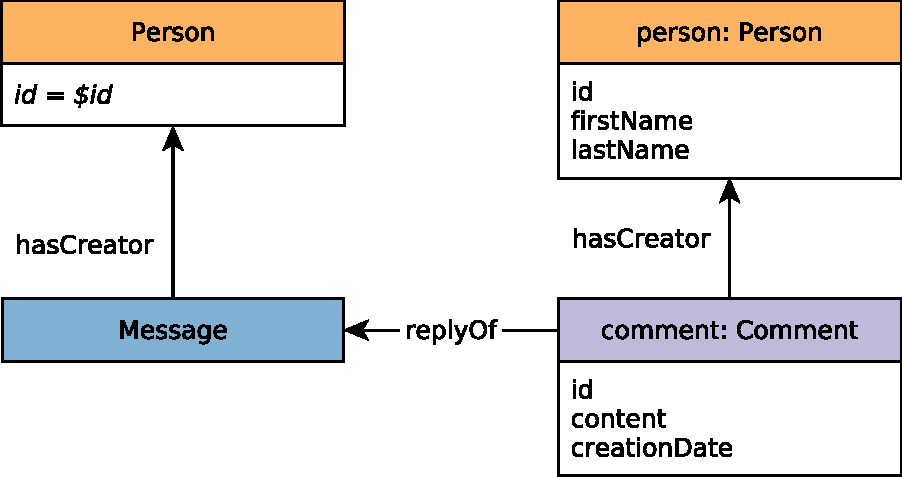
\includegraphics[scale=\patternscale,margin=0cm .2cm]{patterns/interactive08}} \\ \hline
	description & Given a start Person, find (most recent) Comments that are replies to
Messages of the start Person. Only consider immediate (1-hop) replies,
not the transitive (multi-hop) case. Return the reply Comments, and the
Person that created each reply Comment.
 \\ \hline
	
%
	parameters  &
	\vspace{1.1ex}{\begin{tabularx}{14.38cm}{|c|M|m{2cm}|Y} \hline
	\cellcolor{black!70} \color{white} $\mathsf{1}$ & \varname{Person.id} & \cellcolor{gray!20} \vartype{ID} &  \\
	\end{tabularx}} \\ \hline
%
	result      &
	\vspace{1.1ex}{\begin{tabularx}{14.38cm}{|c|M|m{2cm}|Y} \hline
	\cellcolor{black!70} \color{white} $\mathsf{1}$ & \varname{Person.id} & \cellcolor{gray!20} \vartype{ID} &  \\\hline
	\cellcolor{black!70} \color{white} $\mathsf{2}$ & \varname{Person.firstName} & \cellcolor{gray!20} \vartype{String} &  \\\hline
	\cellcolor{black!70} \color{white} $\mathsf{3}$ & \varname{Person.lastName} & \cellcolor{gray!20} \vartype{String} &  \\\hline
	\cellcolor{black!70} \color{white} $\mathsf{4}$ & \varname{Comment.creationDate} & \cellcolor{gray!20} \vartype{DateTime} &  \\\hline
	\cellcolor{black!70} \color{white} $\mathsf{5}$ & \varname{Comment.id} & \cellcolor{gray!20} \vartype{ID} &  \\\hline
	\cellcolor{black!70} \color{white} $\mathsf{6}$ & \varname{Comment.content} & \cellcolor{gray!20} \vartype{String} &  \\
	\end{tabularx}} \\ \hline
	%
	sort        &
	\vspace{1.1ex}{\begin{tabular}{|c|l|c|} \hline
	\cellcolor{black!70} \color{white} $\mathsf{1}$ & \varname{Comment.creationDate} & \cellcolor{gray!20} $\desc$ \\\hline
	\cellcolor{black!70} \color{white} $\mathsf{2}$ & \varname{Comment.id} & \cellcolor{gray!20} $\asc$ \\
	\end{tabular}} \\ \hline
	%
	limit       & 20 \\ \hline
	%
	choke points &
	\multicolumn{1}{>{\raggedright}X|}{
		}\\ \hline
\end{tabularx}
\clearpage